\documentclass[11pt, a4paper]{article}

\usepackage[utf8]{inputenc}
\usepackage[T1]{fontenc}
\usepackage[polish]{babel}
\usepackage{lmodern}
\usepackage[margin=2.5cm]{geometry}
\usepackage{amsmath, amssymb}
\usepackage[normalem]{ulem}
\usepackage{enumitem}
\usepackage{listings}
\usepackage{xcolor}
\usepackage{graphicx}
\usepackage{hyperref}

\lstset{
    basicstyle=\ttfamily\small,
    backgroundcolor=\color{gray!10},
    frame=single,
    breaklines=true,
    extendedchars=true,
    literate={ą}{{\k{a}}}1 {ć}{{\'c}}1 {ę}{{\k{e}}}1 {ł}{{\l{}}}1 {ń}{{\'n}}1 {ó}{{\'o}}1 {ś}{{\'s}}1 {ź}{{\'z}}1 {ż}{{\.z}}1
             {Ą}{{\k{A}}}1 {Ć}{{\'C}}1 {Ę}{{\k{E}}}1 {Ł}{{\L{}}}1 {Ń}{{\'N}}1 {Ó}{{\'O}}1 {Ś}{{\'S}}1 {Ź}{{\'Z}}1 {Ż}{{\.Z}}1
}

\title{Markdown, Colab i GitHub}
\author{}
\date{}

\begin{document}

\maketitle

Na początek poznamy trzy narzędzia, które rozwiązują trzy różne problemy:

\begin{center}
\begin{tabular}{|l|p{10cm}|}
\hline
\textbf{Narzędzie} & \textbf{Do czego służy?} \\ \hline
Markdown & do prostego zapisywania uporządkowanego tekstu, dokumentacji i raportów \\ \hline
Google Colab & do łączenia tekstu, kodu, obliczeń i wyników w jednym notebooku \\ \hline
GitHub & do przechowywania projektu, śledzenia zmian i współpracy \\ \hline
\end{tabular}
\end{center}

Te trzy elementy bardzo dobrze ze sobą współpracują. Podstawą wszędzie jest przygotowanie opisu w kodzie Markdown. Do tego dochodzić będą obliczenia w Colabie, a następnie przechowanie źródła i wyniki w repozytorium GitHub.

\hrulefill

\section{Markdown}

\subsection{Co to jest Markdown?}
Markdown to prosty język znaczników służący do formatowania zwykłego tekstu. Najczęściej zapisujemy go w plikach z rozszerzeniem:
\begin{lstlisting}
.md
\end{lstlisting}

Przykłady:
\begin{lstlisting}
README.md
raport.md
notatki.md
\end{lstlisting}

Plik Markdown jest zwykłym plikiem tekstowym. Można go otworzyć praktycznie w każdym edytorze. Specjalne znaki, takie jak \texttt{\#}, \texttt{*}, \texttt{-} czy \texttt{\$}, informują program wyświetlający dokument, jak ma wyglądać tekst.

\subsection{Dlaczego Markdown jest tak istotny?}
Za każdym razem rozmawiając z chatem AI tak naprawdę rozmawiamy z plikiem Markdown. AI potrafi interpretować składnię Markdown i generować raporty w tym formacie. Dlatego też jak skopiujesz output to ma on całą masę znaczników (np. \texttt{\#}, \texttt{*}, \texttt{-}, czy \texttt{\$}), które są potrzebne do poprawnego renderowania.

GitHub (archiwum programistyczne) zawiera opisy również w Markdown. Podobnie Google Colab (środowisko programistyczne Pythona) potrafi renderować Markdown. Dzięki temu możemy przygotować raport, który będzie wyglądał dobrze zarówno w przeglądarce, jak i w notebooku.

Warto od razu rozróżnić dwie rzeczy:
\begin{itemize}
    \item \textbf{źródło Markdown} — tekst, który wpisujemy do pliku,
    \item \textbf{wyrenderowany dokument} — wygląd tego tekstu po interpretacji składni Markdown.
\end{itemize}

Na GitHubie możemy przełączać się między widokiem źródła i wyrenderowanym dokumentem. Podobnie edytory kodu jak VS Code, PyCharm czy Jupyter Notebook potrafią renderować Markdown w osobnym oknie podglądu.

Zanim zaczniemy pisać w Markdown zobacz przykładowy plik Markdown. Raport na temat ciała na sprężynie: ,,Ciało na sprężynie''.

\subsection{Nagłówki}
Nagłówki budują strukturę dokumentu. Im więcej znaków \texttt{\#}, tym niższy poziom nagłówka.

\textbf{Źródło:}
\begin{lstlisting}
# Tytuł dokumentu

## Główna sekcja

### Podsekcja
\end{lstlisting}

\textbf{Efekt:}
\begin{quote}
{\Large\bfseries Tytuł dokumentu}\\[0.5em]
{\large\bfseries Główna sekcja}\\[0.4em]
{\normalsize\bfseries Podsekcja}
\end{quote}

W praktyce jeden dokument powinien mieć jeden główny nagłówek \texttt{\#}. Dalsze części dokumentu organizujemy za pomocą \texttt{\#\#}, \texttt{\#\#\#} itd.

\hrulefill

\subsection{Pogrubienie, kursywa i przekreślenie}
\textbf{Źródło:}
\begin{lstlisting}
**tekst pogrubiony**

*tekst pochylony*

~~tekst przekreślony~~

***tekst pogrubiony i pochylony***
\end{lstlisting}

\textbf{Efekt:}
\begin{itemize}[label={}, leftmargin=0pt]
    \item \textbf{tekst pogrubiony}
    \item \textit{tekst pochylony}
    \item \sout{tekst przekreślony}
    \item \textbf{\textit{tekst pogrubiony i pochylony}}
\end{itemize}

Wyróżnień warto używać oszczędnie. Jeśli wszystko jest pogrubione, nic nie jest naprawdę wyróżnione.

\hrulefill

\subsection{Akapit i nowa linia}
Nowy akapit tworzymy przez pozostawienie pustej linii.

\textbf{Źródło:}
\begin{lstlisting}
To jest pierwszy akapit.

To jest drugi akapit.
\end{lstlisting}

\textbf{Efekt:}

To jest pierwszy akapit.

To jest drugi akapit.

To ważna zasada: w Markdown pojedyncze naciśnięcie Enter nie zawsze oznacza nowy akapit.

\hrulefill

\subsection{Listy punktowane}
\textbf{Źródło:}
\begin{lstlisting}
- Markdown
- Colab
- GitHub
\end{lstlisting}

\textbf{Efekt:}
\begin{itemize}
    \item Markdown
    \item Colab
    \item GitHub
\end{itemize}

Listy można zagnieżdżać:
\begin{lstlisting}
- GitHub
  - repozytorium
  - Issues
  - historia zmian
- Colab
  - tekst
  - kod
  - wyniki
\end{lstlisting}

\textbf{Efekt:}
\begin{itemize}
    \item GitHub
    \begin{itemize}
        \item repozytorium
        \item Issues
        \item historia zmian
    \end{itemize}
    \item Colab
    \begin{itemize}
        \item tekst
        \item kod
        \item wyniki
    \end{itemize}
\end{itemize}

\hrulefill
\subsection{Listy numerowane}
\textbf{Źródło:}
\begin{lstlisting}
1. przygotuj dane,
2. wykonaj obliczenia,
3. zapisz wynik,
4. opisz wynik.
\end{lstlisting}

\textbf{Efekt:}
\begin{enumerate}
    \item przygotuj dane,
    \item wykonaj obliczenia,
    \item zapisz wynik,
    \item opisz wynik.
\end{enumerate}

Listy numerowane są szczególnie przydatne przy opisie procedury lub instrukcji.

\hrulefill

\subsection{Checklisty}
GitHub obsługuje listy zadań.

\textbf{Źródło:}
\begin{lstlisting}
- [x] utworzono notebook
- [x] wykonano obliczenia
- [ ] sprawdzono wynik
\end{lstlisting}

\textbf{Efekt:}
\begin{itemize}
    \item[$\boxtimes$] utworzono notebook
    \item[$\boxtimes$] wykonano obliczenia
    \item[$\square$] sprawdzono wynik
\end{itemize}

Checklisty bardzo dobrze nadają się do krótkich list kontrolnych w dokumentacji i GitHub Issues.

\hrulefill

\subsection{Linki}
\textbf{Źródło:}
\begin{lstlisting}
[GitHub](https://github.com/)
\end{lstlisting}

\textbf{Efekt:} \href{https://github.com/}{GitHub}

Zamiast wklejać długi adres do strony, warto umieścić go pod czytelną nazwą.

\hrulefill

\subsection{Obrazy}
Obraz osadzamy podobnie jak link, ale na początku dodajemy znak \texttt{!}.

\textbf{Źródło:}
\begin{lstlisting}
![Wykres zależności y od x](wykres.png)
\end{lstlisting}

Jeżeli plik \texttt{wykres.png} znajduje się w tym samym folderze co dokument Markdown, GitHub wyświetli obraz w miejscu tej instrukcji. Jeżeli plik znajduje się w podfolderze \texttt{files}, używamy ścieżki:
\begin{lstlisting}
![Wykres zależności y od x](files/wykres.png)
\end{lstlisting}

\textbf{Efekt:}
\begin{figure}[h]
    \centering
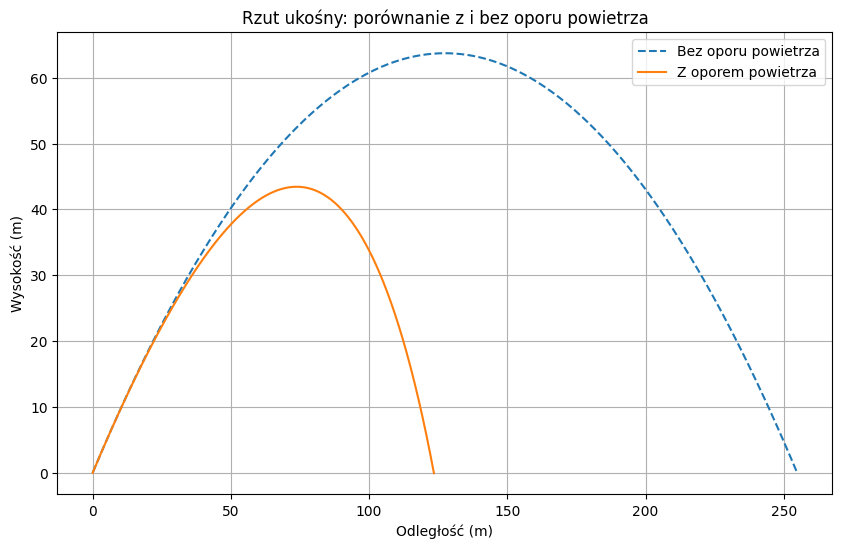
\includegraphics[width=0.5\textwidth]{wykres.png}
    \caption{Wykres zależności y od x}
\end{figure}

Tekst w nawiasach kwadratowych jest opisem obrazu. Warto go uzupełniać — pomaga zrozumieć zawartość także wtedy, gdy obraz nie może zostać wyświetlony. W projektach przechowywanych w repozytorium zwykle wygodniej używać ścieżek względnych niż pełnych adresów internetowych.

\hrulefill

\subsection{Tabele}
\textbf{Źródło:}
\begin{lstlisting}
| Narzędzie | Typ pliku | Zastosowanie |
| --- | --- | --- |
| Markdown | .md | dokumentacja |
| Colab | .ipynb | obliczenia |
| GitHub | repozytorium | historia projektu |
\end{lstlisting}

\textbf{Efekt:}
\begin{center}
\begin{tabular}{|l|l|l|}
\hline
\textbf{Narzędzie} & \textbf{Typ pliku} & \textbf{Zastosowanie} \\ \hline
Markdown & \texttt{.md} & dokumentacja \\ \hline
Colab & \texttt{.ipynb} & obliczenia \\ \hline
GitHub & repozytorium & historia projektu \\ \hline
\end{tabular}
\end{center}

Tabele są dobre do krótkich zestawień. Jeśli w komórkach pojawiają się długie akapity tekstu, zwykle lepiej wrócić do zwykłych sekcji i list.

\hrulefill

\subsection{Kod w tekście}
Nazwy plików, komendy i bardzo krótkie fragmenty kodu warto oznaczać pojedynczym backtickiem.

\textbf{Źródło:}
\begin{lstlisting}
Uruchom plik `analiza.py` i sprawdź wartość zmiennej `wynik`.
\end{lstlisting}

\textbf{Efekt:} Uruchom plik \texttt{analiza.py} i sprawdź wartość zmiennej \texttt{wynik}.

\hrulefill

\subsection{Bloki kodu}
Większy fragment kodu umieszczamy w osobnym bloku. Podanie nazwy języka, np. \texttt{python}, \texttt{bash}, \texttt{html} czy \texttt{json}, pozwala GitHubowi kolorować składnię.

\textbf{Efekt:}
\begin{lstlisting}[language=Python]
x = 5
y = x**2
print(y)
\end{lstlisting}

W raporcie technicznym dobrze jest pokazać krótki fragment kodu, który jest istotny dla opisywanego wyniku. Nie trzeba kopiować do raportu całego programu.

\hrulefill

\subsection{Cytaty}
\textbf{Źródło:}
\begin{lstlisting}
> Wynik należy zawsze sprawdzić przed jego wykorzystaniem.
\end{lstlisting}

\textbf{Efekt:}
\begin{quote}
\itshape Wynik należy zawsze sprawdzić przed jego wykorzystaniem.
\end{quote}

Cytaty można wykorzystać także do krótkiego wyróżnienia komentarza lub uwagi.

\hrulefill

\subsection{Matematyka}
GitHub potrafi renderować wzory matematyczne. Krótki wzór umieszczamy wewnątrz pojedynczych znaków dolara.

\textbf{Źródło:}
\begin{lstlisting}
Energia spoczynkowa dana jest wzorem $E=mc^2$.
\end{lstlisting}

\textbf{Efekt:} Energia spoczynkowa dana jest wzorem $E=mc^2$.

Dłuższy wzór umieszczamy w osobnym bloku.

\textbf{Źródło:}
\begin{lstlisting}
$$
\sum_{k=1}^{n} k^2 = \frac{n(n+1)(2n+1)}{6}
$$
\end{lstlisting}

\textbf{Efekt:}
$$
\sum_{k=1}^{n} k^2 = \frac{n(n+1)(2n+1)}{6}
$$

Macierze zapisujemy wielowierszowo:
\begin{lstlisting}
$$
A=
\begin{pmatrix}
1 & 2 \\
3 & 4 \\
\end{pmatrix}
$$
\end{lstlisting}

\textbf{Efekt:}
$$
A=
\begin{pmatrix}
1 & 2 \\
3 & 4 \\
\end{pmatrix}
$$

\hrulefill

\subsection{Zrzut ekranu i transkrypcja do Markdown}
Czasem informacja istnieje tylko jako obraz: zrzut ekranu programu, zdjęcie tabeli, komunikat błędu albo fragment zeskanowanego dokumentu. AI może pomóc przepisać zawartość obrazu do tekstu. Taki proces nazywamy tutaj transkrypcją.

Przykładowy workflow:
\begin{enumerate}
    \item zachowujemy oryginalny obraz,
    \item prosimy AI o przepisanie jego zawartości do kodu markdown,
    \item zapisujemy wynik w pliku tekstowym lub Markdown,
    \item porównujemy transkrypcję z obrazem,
    \item poprawiamy ewentualne błędy.
\end{enumerate}

Największej ostrożności wymagają:
\begin{itemize}
    \item liczby,
    \item wzory,
    \item nazwy plików,
    \item adresy,
    \item fragmenty kodu,
    \item komunikaty błędów.
\end{itemize}

Transkrypcja wygenerowana przez AI jest wersją roboczą, dopóki człowiek jej nie sprawdzi.

\hrulefill

\subsection{Poprawne formatowanie matematyki w Markdown}
W materiałach tego kursu polecamy stosowanie prostego zestawu reguł formatowania matematyki przygotowanego specjalnie tak, aby pliki dobrze renderowały się na GitHubie: \texttt{hints.md}. Pracując z chatem AI i domagając się kodu markdowna, warto załączać ten plik jako kontekst, aby AI od razu generowało poprawny kod w Markdown.

Różne systemy: przeglądarkowe chaty AI, Edytor Visual Studio, Colab i GitHub, mogą różnie renderować wzory matematyczne! Częstym błędem jest używanie w kodzie Markdown znaków \texttt{\textbackslash[]} i \texttt{\textbackslash]} zamiast \texttt{\$ \$} do oznaczania wzorów matematycznych. Wtedy GitHub nie renderuje wzoru, a Colab renderuje go poprawnie.

\hrulefill

\subsection{Dobre materiały o Markdown}
\begin{itemize}
    \item \href{https://docs.github.com/en/get-started/writing-on-github/getting-started-with-writing-and-formatting-on-github/basic-writing-and-formatting-syntax}{GitHub Docs — Basic writing and formatting syntax}
    \item \href{https://docs.github.com/en/get-started/writing-on-github/working-with-advanced-formatting/writing-mathematical-expressions}{GitHub Docs — Writing mathematical expressions}
    \item \href{https://www.markdownguide.org/basic-syntax/}{Markdown Guide — Basic Syntax}
    \item \href{https://www.markdownguide.org/cheat-sheet/}{Markdown Guide — Cheat Sheet}
\end{itemize}

\end{document}